\documentclass[a4paper,10pt]{article}

\usepackage{amsmath}
%\usepackage[utf8]{inputenc} % pour les accents
\usepackage[T1]{fontenc} % caracteres francais
\usepackage{geometry} %les marges
\usepackage[french]{babel} %langue principale
\usepackage[dvips]{graphicx}
\usepackage{textcomp}
\geometry{ hmargin=2cm, vmargin=2cm }

\pagestyle{empty} %pas de numerotation de page

%
% Debut du document
%
\begin{document}

\section*{FICHE DE VALIDATION DU LOGICIEL MASCARET V7P2}

\subsection*{Validation du noyau transcritique}

\subsection*{\emph{Prise en compte de termes non hydrostatiques}}

\subsection*{Num�ro du cas test : 28}

\subsection*{Auteur : Nicole GOUTAL - Fabrice ZAOUI}

\vspace{1cm}

\subsection*{Description}

Il s'agit de v�rifier la capacit� du noyau transcritique � tenir compte de termes non-hydrostatiques pour mod�liser les ondes de Favre.
Ces ondes secondaires apparaissent lors d'une variation brusque de d�bit dans un canal et se pr�sentent sous la forme d'ondulations se superposant au corps de l'onde de Saint-Venant.

\subsection*{Donn�es g�om�triques}

Le calcul concerne un canal rectangulaire de longueur $30\ m$ et de largeur $40\ cm$ avec une pente de $4$\textperthousand.

\subsection*{Donn�es physiques}

Le coefficient de rugosit� est choisi de mani�re � ce que la hauteur normale soit $h_n = 0.2\ m$ d'o� une valeur : $K = 102 m^{1/3}.s^{-1}$ (application de la formule de Strickler).

\vspace{0.5cm}

\begin{itemize}
  \item Conditions initiales :
  \begin{itemize}
    \item le r�gime permanent correspondant � la hauteur normale $h_n$.
  \end{itemize}
  \item Conditions aux limites :
  \begin{itemize}
     \item un hydrogramme constant � l'omont;
     \item un hydrogramme pour simuler un d�clenchement de d�bit � l'aval sur un temps tr�s court de $0.07\ s$ .
  \end{itemize}
\end{itemize}

\subsection*{Donn�es num�riques}

Le maillage a un pas d'espace de $5\ cm$.

Le pas de planim�trage est homog�ne dans le domaine �gal � $1\ cm$.

Le calcul est effectu� sur une p�riode de $6\ s$ avec un pas de temps initial de $0.01\ s$ et un nombre de Courant souhait� de $0.8$.


\subsection*{R�sultats}

La figure \ref{fig1} pr�sente les r�sultats de calcul avec et sans prise en compte des termes non hydrostatiques en comparaison de mesures exp�rimentales � $2\ m$ de l'aval du domaine.

\begin{figure}[h]
 \begin{center}
  \includegraphics[angle=270,width=12cm]{Fig1.eps}
  \caption{Evolutions de la cote d'eau en $x = 28\ m$}
  \label{fig1}
 \end{center}
\end{figure}

\subsection*{Conclusion}

La prise en compte des termes non hydrostatiques mod�lise bien les ondes de Favre se superposant au corps d'onde de Saint-Venant (toujours v�rifier ce point). L'amplitude calcul�e est moindre et l'amortissement plus rapide en comparaison des donn�es exp�rimentales. Un sch�ma d'ordre plus elev� tend � corriger ce probl�me \cite{BRISTEAU11}.

\begin{thebibliography}{1}

\bibitem{BRISTEAU11} M.-O. BRISTEAU, N. GOUTAL and J. SAINTE-MARIE \emph{Numerical simulations of a non-hydrostatic shallow water model}, Computers \& Fluids, vol. 47, pp. 51-64, 2011

\end{thebibliography}
%
% fin du document
%
\end{document}          
